\begin{center}
    \large\textbf{大学生``容貌焦虑''情况调查问卷}
\end{center}
\begin{enumerate}[label=第\arabic{*}题、, leftmargin=7em]
    \item 您的性别是
    \begin{enumerate}[label=\Alph*.]
        \item 男
        \item 女
    \end{enumerate}

    \item 您所在的年级
    \begin{enumerate}[label=\Alph*.]
        \item 大一
        \item 大二
        \item 大三及以上本科
        \item 硕士
        \item 博士
    \end{enumerate}

    \item 下列哪一个最符合您的审美(对于男生)
    \setcounter{subfigure}{0}
    \begin{figure}[H]
        \centering
        \subfigure[A选项图]{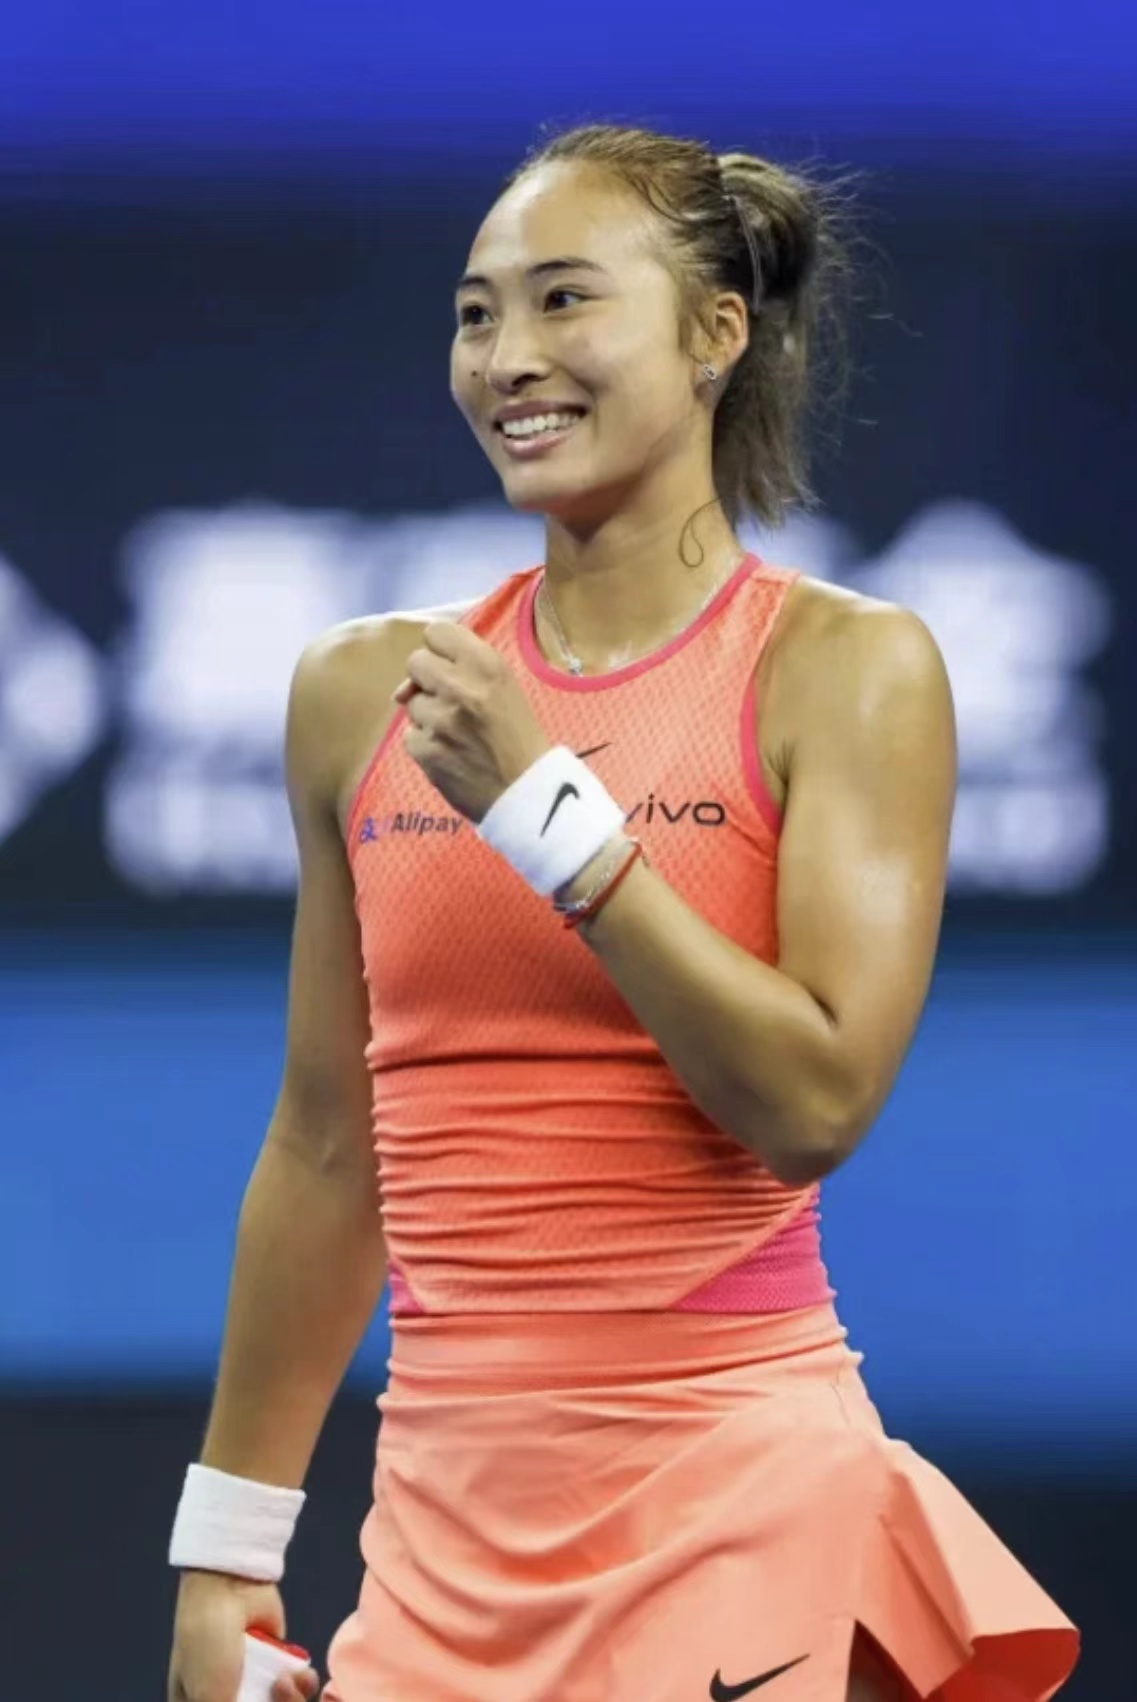
\includegraphics[width=0.15\textwidth]{./assets/T2-1.jpg}}
        \subfigure[B选项图]{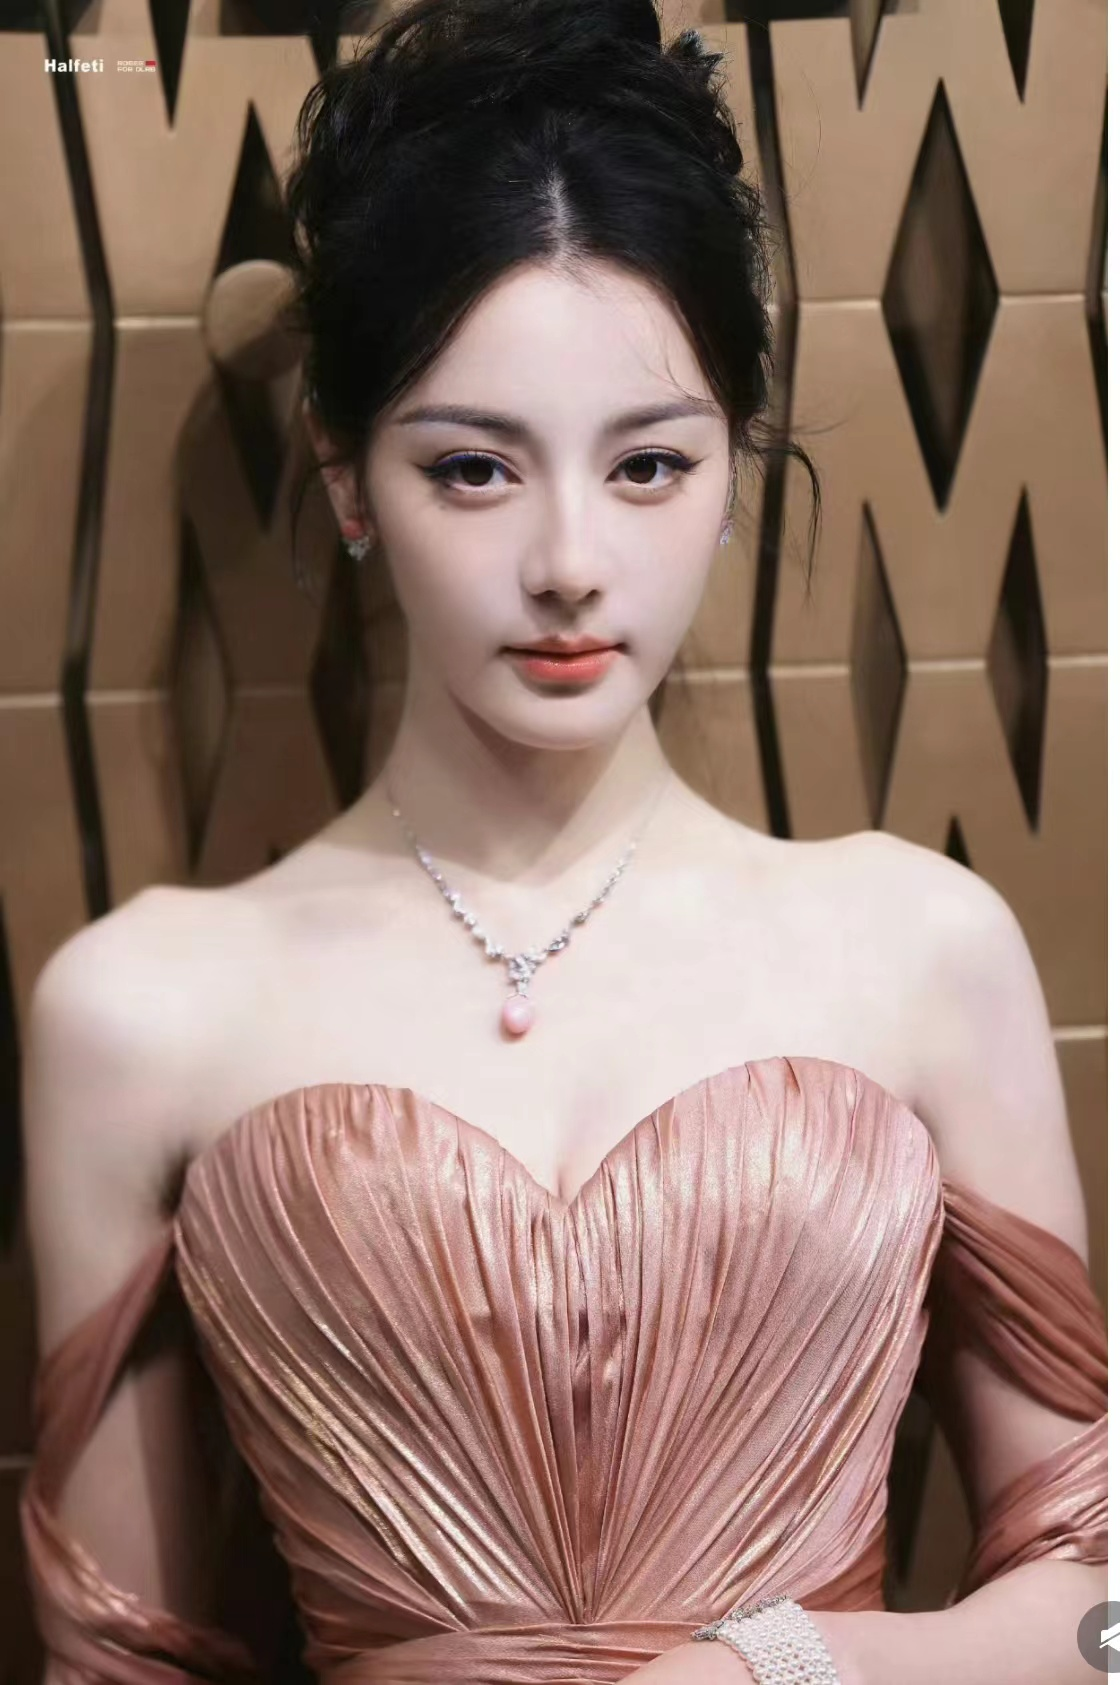
\includegraphics[width=0.15\textwidth]{./assets/T2-2.jpg}}
        \subfigure[C选项图]{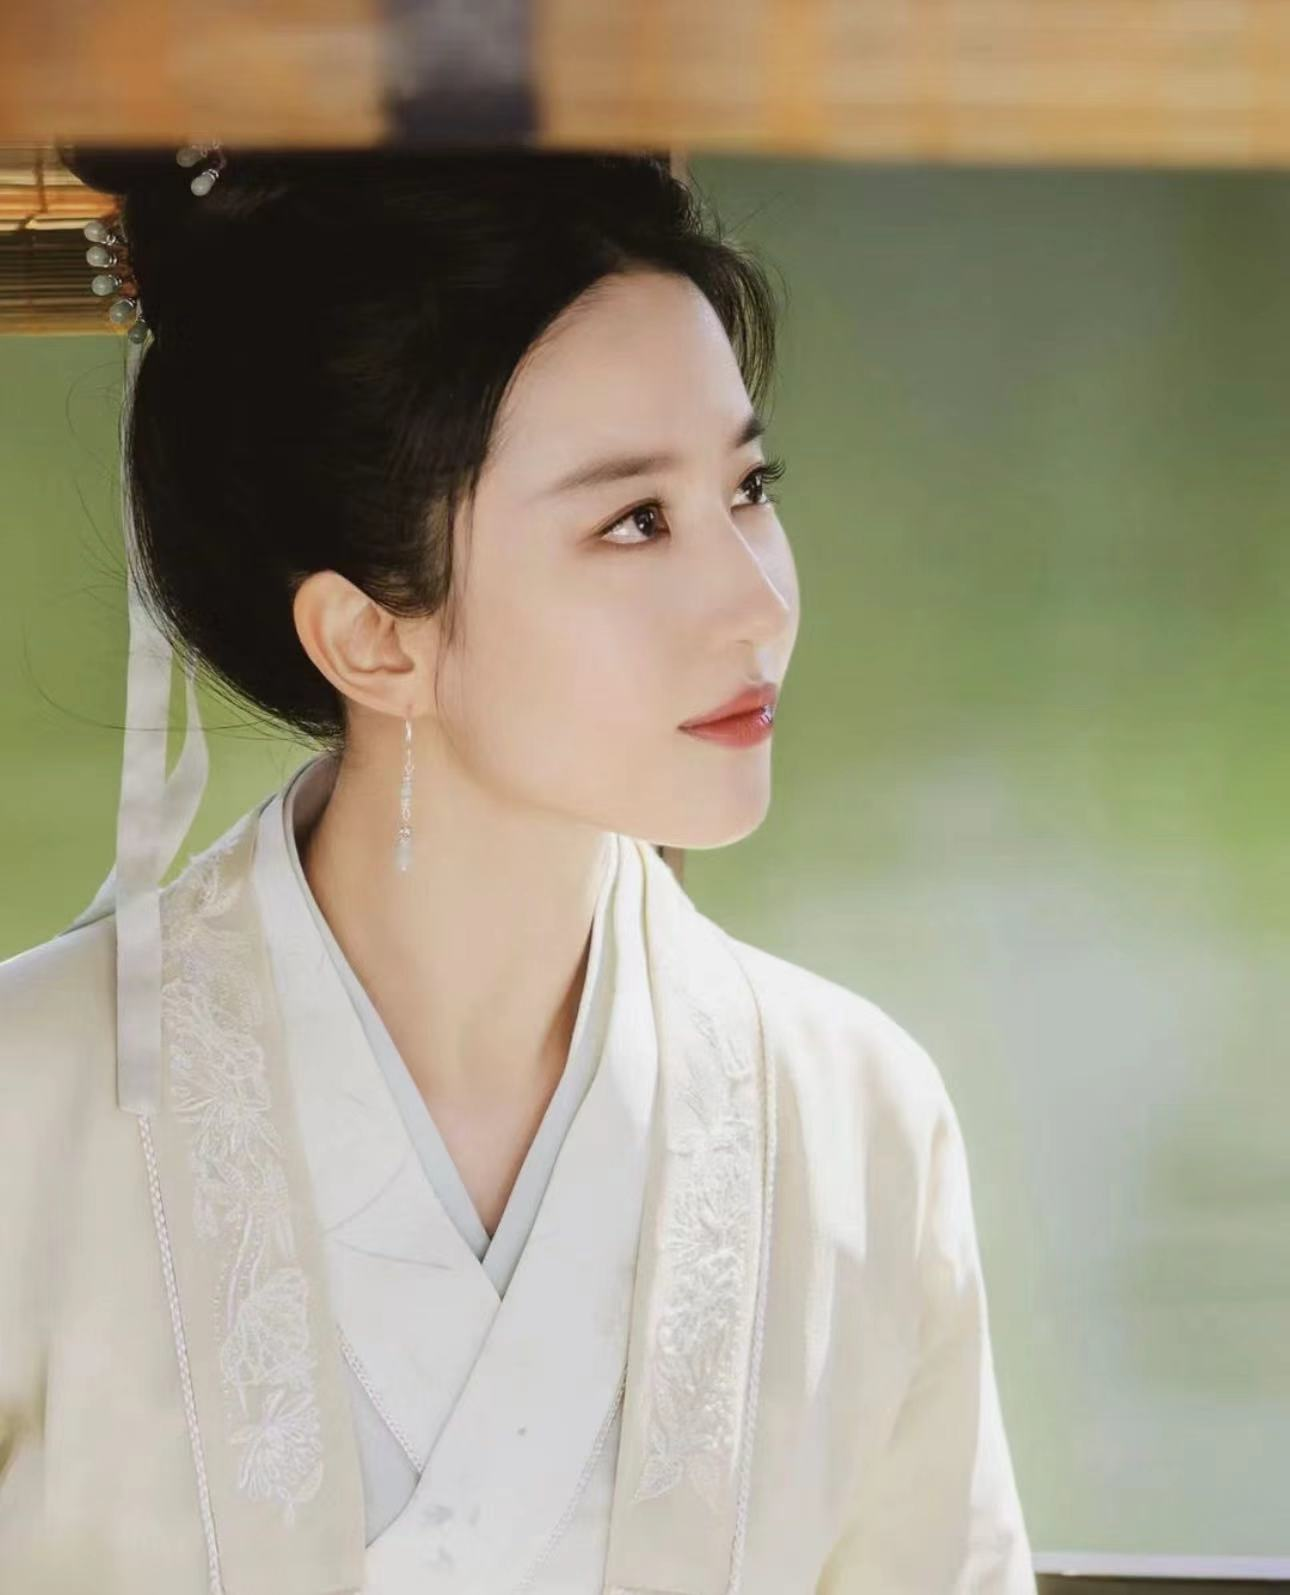
\includegraphics[width=0.15\textwidth]{./assets/T2-3.jpg}}
    \end{figure}



    \item 下列哪一个最符合您的审美(对于女生)
    \setcounter{subfigure}{0}
    \begin{figure}[H]
        \centering
        \subfigure[A选项图]{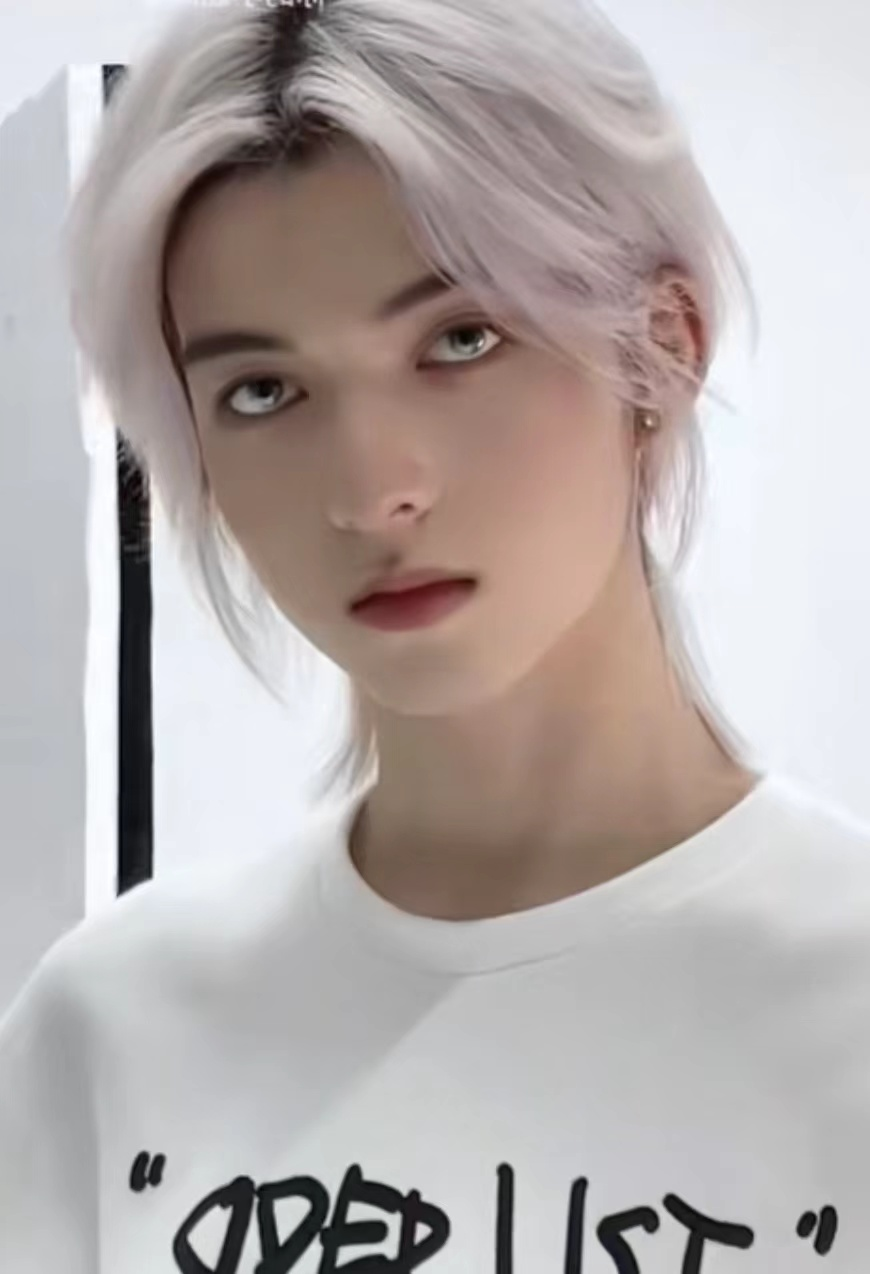
\includegraphics[width=0.15\textwidth]{./assets/T2-4.jpg}}
        \subfigure[B选项图]{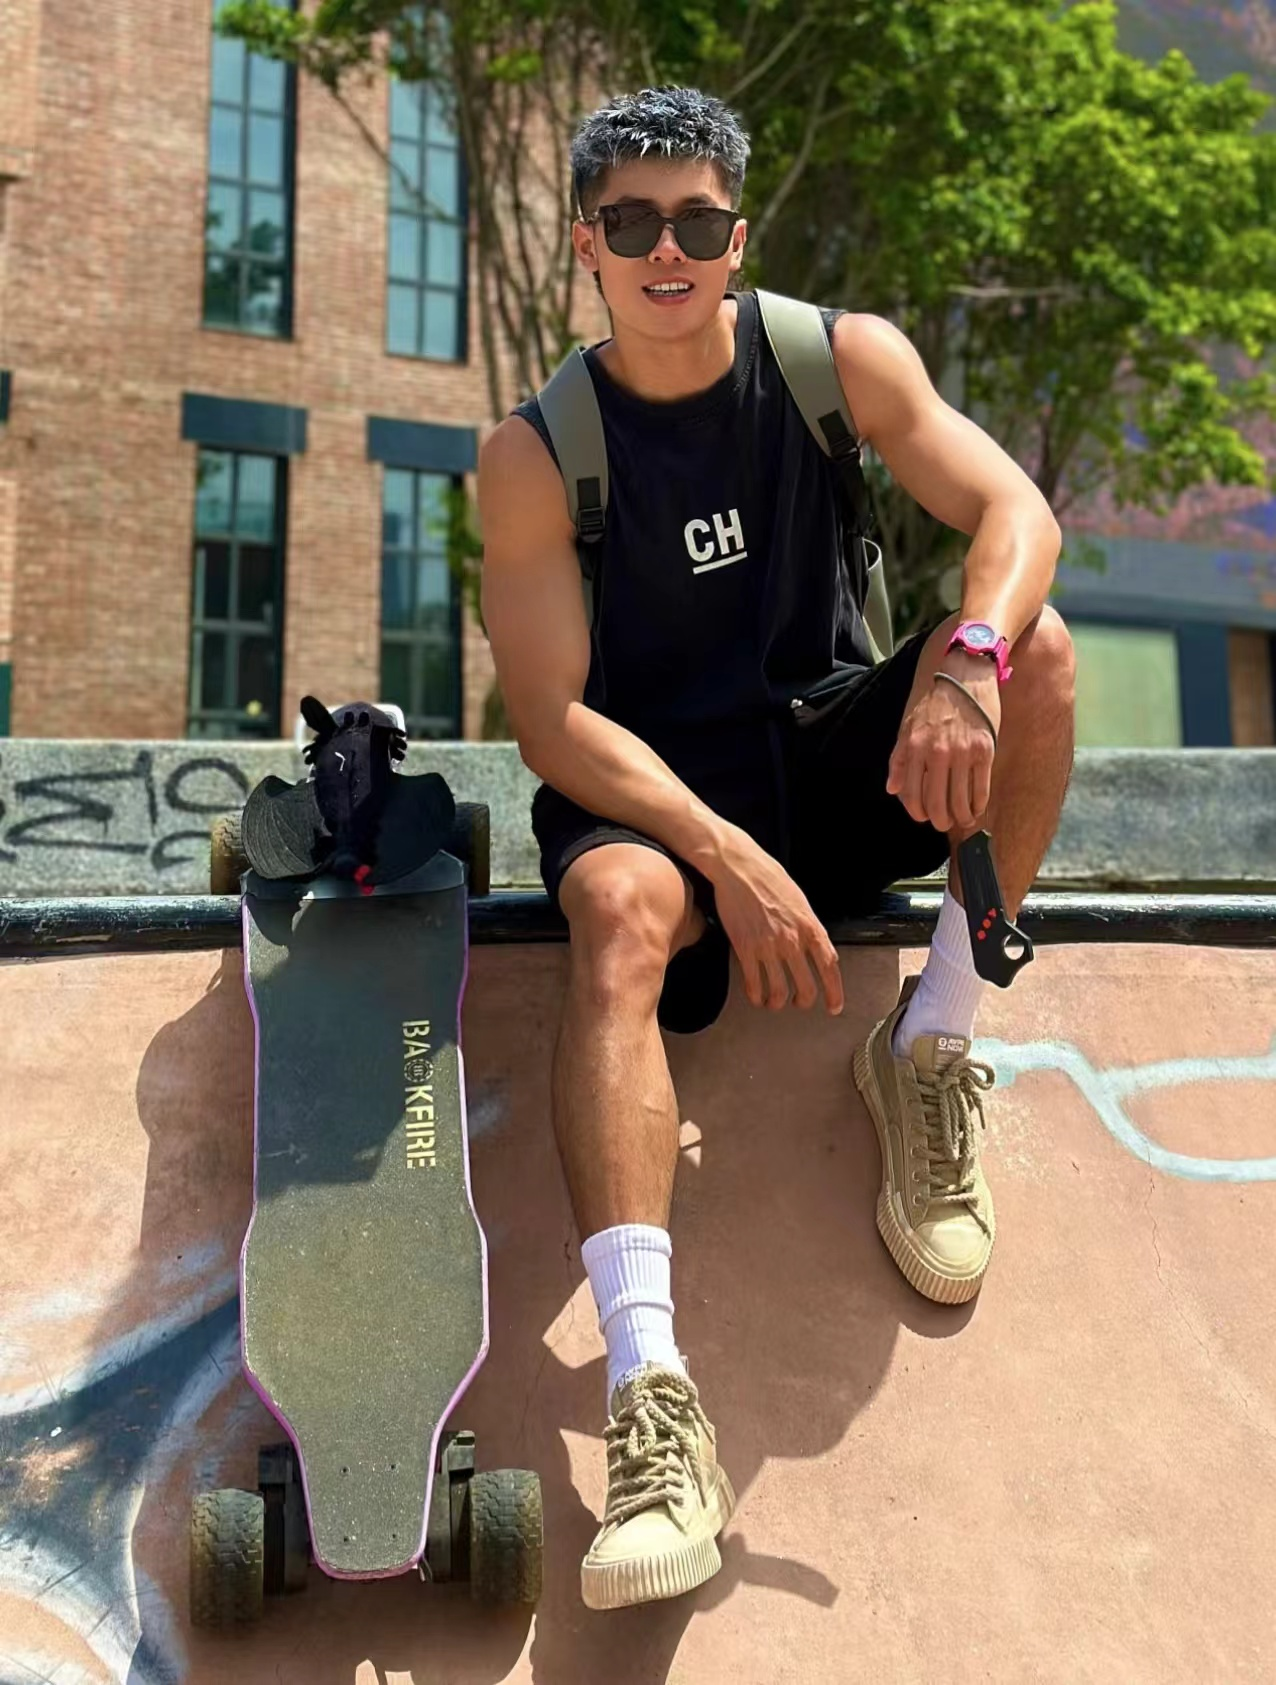
\includegraphics[width=0.15\textwidth]{./assets/T2-5.jpg}}
        \subfigure[C选项图]{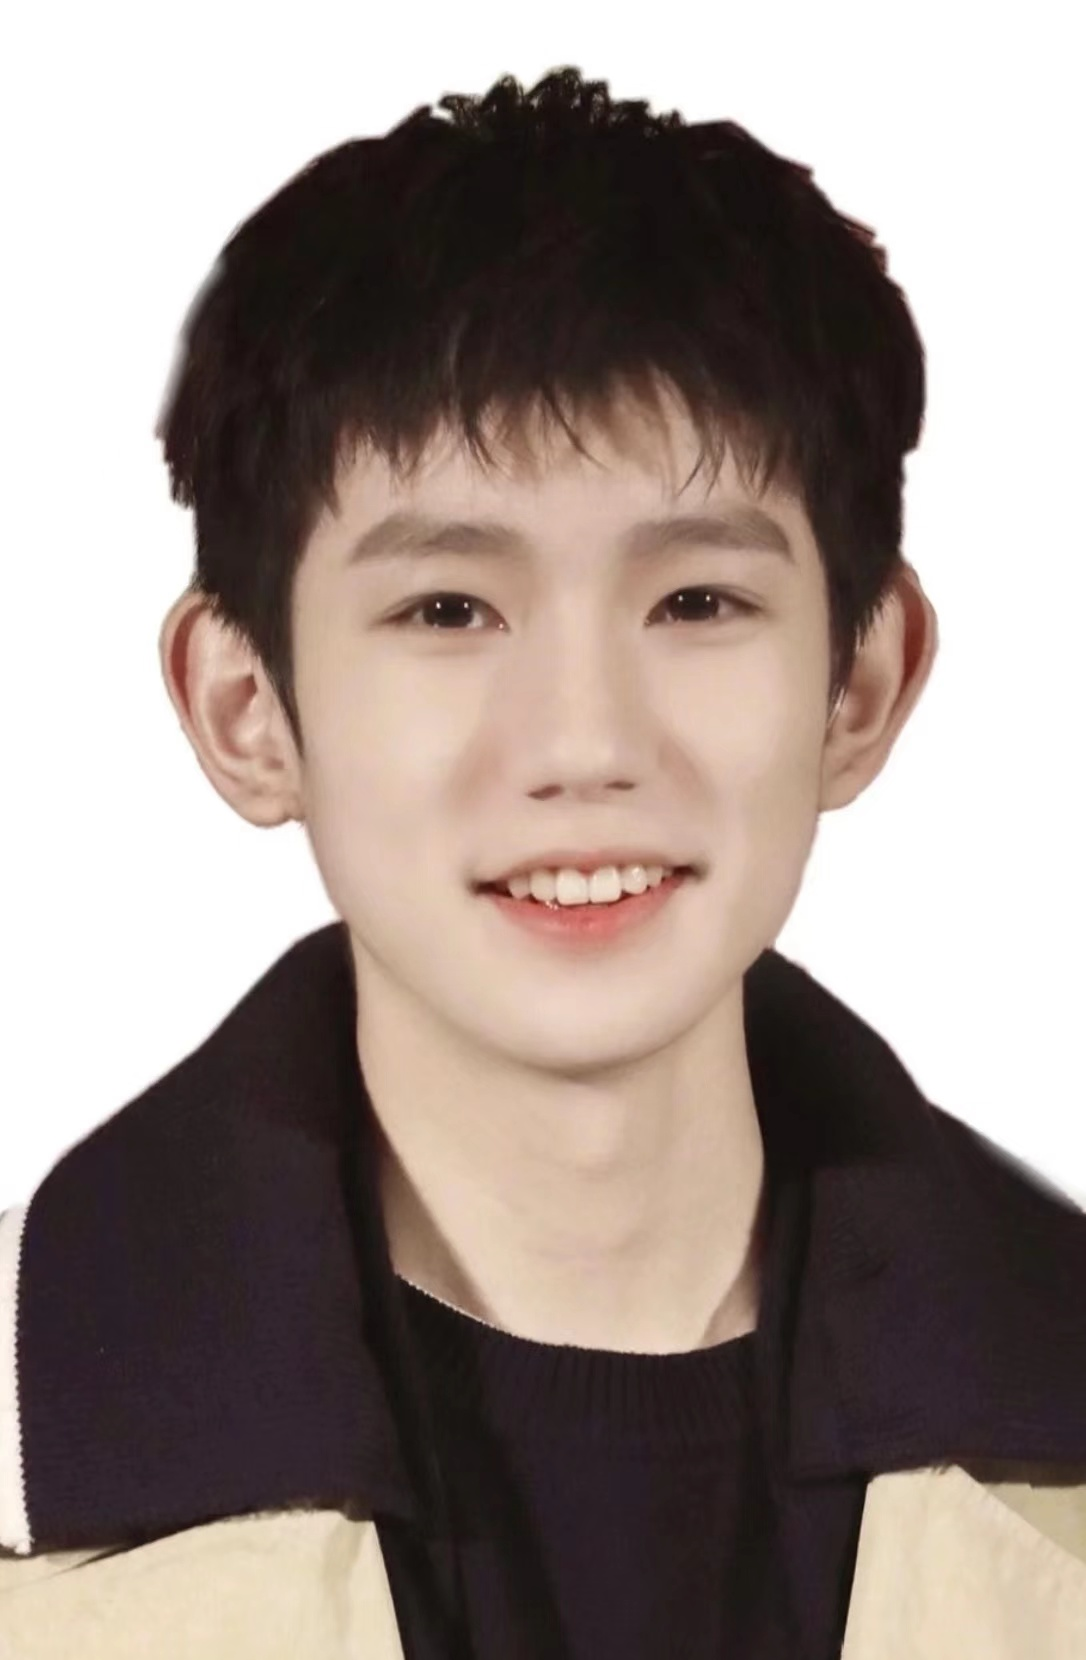
\includegraphics[width=0.15\textwidth]{./assets/T2-6.jpg}}
    \end{figure}



    \item 在你的家庭生活中,以下哪些方面体现了美学文化?
    \begin{enumerate}[label=\Alph*.]
        \item 家居布置注重色彩搭配和协调
        \item 家庭成员有欣赏艺术作品(绘画、音乐等)的习惯
        \item 日常饮食注重摆盘美观
        \item 家庭活动有一定的仪式感和美感设计
        \item 家庭成员的穿着打扮具有时尚感和审美品味
        \item 家庭布置有盆栽,花卉等设计
        \item 日常不太注意
        \item 其他
    \end{enumerate}

    \item 对于化妆、医美,您的看法是
    \begin{enumerate}[label=\Alph*.]
        \item 无法理解他人频繁医美或化妆的行为,但是适度可以
        \item 个人喜好,开心就好,不管程度如何,外人无权干涉
        \item 对医美和化妆行为表示不解
        \item 如果不考虑成本等其他因素,会尝试化妆
        \item 如果不考虑本等其他因素,会尝试医美
    \end{enumerate}

    \item 您每天会花费多少时间在修饰自身容貌上
    \begin{enumerate}[label=\Alph*.]
        \item <1.5h
        \item 1.5h$\sim $3h
        \item >3h
    \end{enumerate}

    \item 如何看待花费时间精力在整理容貌这个事情
    \begin{enumerate}[label=\Alph*.]
        \item 爱美之心人皆有之,我觉得这件事可以改善我的精神面貌
        \item 对时间管理和心理带来了负面的影响,我觉得这可能不是一件好事情
    \end{enumerate}

    \item 如果把``对容貌的关注''认作是有意义的,那您认为他的意义主要在于
    \begin{enumerate}[label=\Alph*.]
        \item 取悦自己,改善精神面貌
        \item 一般社交
        \item 交友
        \item 恋爱
        \item 提升在社会中的竞争力
        \item 其他
    \end{enumerate}

    \item 是什么使您不得不花费大量时间在关注,修饰自身容貌上呢
    \begin{enumerate}[label=\Alph*.]
        \item 网络上通过技术手段来变美的人给你造成容貌上的压力
        \item 受到了医美广告,化妆广告及网红言论,视频的观点影响
        \item 大学时期恋爱导致的容貌需求
        \item 社会竞争压力增大,希望通过容貌的突出来获得一些优势
        \item 其他
    \end{enumerate}

    \item 您面对这些烦恼,有试着用一些办法解决吗
    \begin{enumerate}[label=\Alph*.]
        \item 让自己变忙起来,分散注意力
        \item 减少社交媒体的使用
        \item 将关注的重点从外在容貌改到内在品质
        \item 没有尝试
    \end{enumerate}

    \item 这些办法的效果如何呢?
    \begin{enumerate}[label=\Alph*.]
        \item 很有效果
        \item 没有用,依然想要解决这些烦恼
        \item 经过一段时间,觉得维持现状也挺好,不必打破内心与生活的平衡

    \end{enumerate}
    \item 您认为以下哪些情况是``容貌焦虑''的表现?
    \begin{enumerate}[label=\Alph*.]
        \item 怎么看自己都觉得胖、丑、奇怪
        \item 对自己外貌要求严格、苛刻
        \item 用过度或者不健康的方式实现理想外表
        \item 反复拿自己与他人对比
        \item 对自己的外形、体重有很强的不满甚至厌恶情绪
        \item 总想要改变自己的外表
        \item 很在乎别人会怎么看你
        \item 害怕拍照、担心别人看到自己外表的不足
        \item 花费大量时间在关注、修饰容貌上
        \item 素颜遇到crush不敢抬头
        \item 不好意思穿着随意出门
    \end{enumerate}

    \item 可以留下您的联系方式吗?(非必填)

\end{enumerate}